% This file was created by matlab2tikz.
%
%The latest updates can be retrieved from
%  http://www.mathworks.com/matlabcentral/fileexchange/22022-matlab2tikz-matlab2tikz
%where you can also make suggestions and rate matlab2tikz.
%
\documentclass[tikz]{standalone}
\usepackage[T1]{fontenc}
\usepackage[utf8]{inputenc}
\usepackage{pgfplots}
\usepackage{grffile}
\pgfplotsset{compat=newest}
\usetikzlibrary{plotmarks}
\usetikzlibrary{arrows.meta}
\usepgfplotslibrary{patchplots}
\usepackage{amsmath}

\begin{document}
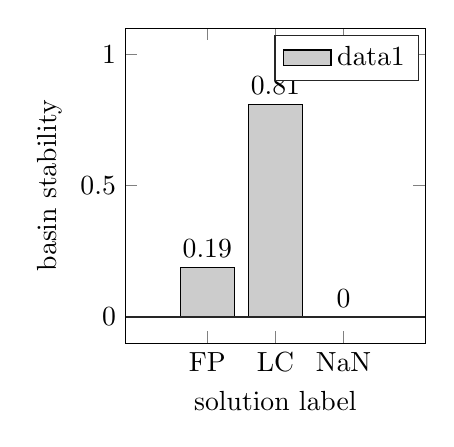
\begin{tikzpicture}

\begin{axis}[%
width=3.804cm,
height=4cm,
at={(0cm,0cm)},
scale only axis,
bar shift auto,
xmin=-0.2,
xmax=4.2,
xtick={1,2,3},
xticklabels={{FP},{LC},{NaN}},
xlabel style={font=\color{white!15!black}},
xlabel={solution label},
ymin=-0.1,
ymax=1.1,
ylabel style={font=\color{white!15!black}},
ylabel={basin stability},
axis background/.style={fill=white},
legend style={legend cell align=left, align=left, draw=white!15!black},
title style={font=\normalsize},xlabel style={font=\normalsize},ylabel style={font=\normalsize},ticklabel style={font=\normalsize}
]
\addplot[ybar, bar width=0.8, fill=white!80!black, draw=black, area legend] table[row sep=crcr] {%
1	0.189\\
2	0.811\\
3	0\\
};
\addplot[forget plot, color=white!15!black, line width=1.0pt] table[row sep=crcr] {%
-0.2	0\\
4.2	0\\
};
\addlegendentry{data1}

\node[above, align=center]
at (axis cs:1,0.189) {0.19};
\node[above, align=center]
at (axis cs:2,0.811) {0.81};
\node[above, align=center]
at (axis cs:3,0) {0};
\end{axis}
\end{tikzpicture}%
\end{document}